%versi 3 (22-07-2020)
\chapter{Landasan Teori}
\label{chap:teori}

\section{Kurikulum 2018}
Kurikulum didefinisikan sebagai seperangkat rencana dan pengaturan mengenai capaian pembelajaran lulusan, bahan kajian, proses, dan penilaian yang digunakan sebagai pedoman penyelenggaraan program studi menjadi sarana utama untuk mencapai tujuan tersebut. \cite{kurikulum:2018}

Penyusunan Kurikulum 2018 berpegang pada prinsip bahwa kurikulum yang baik adalah kurikulum yang tidak hanya kokoh, secara teoretis konseptual dapat dipertanggungjawabkan, namun juga secara praktis dapat dilaksanakan. Selain itu kurikulum juga harus cukup fleksibel agar dapat mengakomodasi perubahan-perubahan, namun tanpa kehilangan ciri atau kekhasan dari program studi.

Dalam penyusunan Kurikulum 2018 Program Studi Teknik Informatika secara khusus juga memperhatikan Kerangka Kualifikasi Nasional Indonesia (KKNI) yang tertuang dalam Peraturan Presiden no 8 tahun 2012. KKNI merupakan pernyataan kualitas SDM Indonesia, di mana tolok ukur kualifikasinya ditetapkan berdasarkan capaian pembelajaran (learning outcomes) yang dimilikinya. Penyusunan kurikulum mengikuti tahapan perancangan kurikulum yang disarankan oleh Kemenristekdikti yang diberikan pada Gambar
\ref{fig:gambar1}. Tahapan penyusunan kurikulum 2018 meliputi kegiatan sebagai berikut:

\begin{enumerate}
    \item Melakukan evaluasi diri
    \item Merumuskan profil lulusan dengan pelacakan lulusan
    \item Menentukan capaian pembelajaran
    \item Menentukan bahan kajian
    \item Menyusun matriks pembelajaran dan bahan kajian
    \item Membentuk mata kuliah
    \item Menyusun struktur kurikulum dan menentukan metode pembelajaran
\end{enumerate}

\begin{figure}[H]
    \centering
    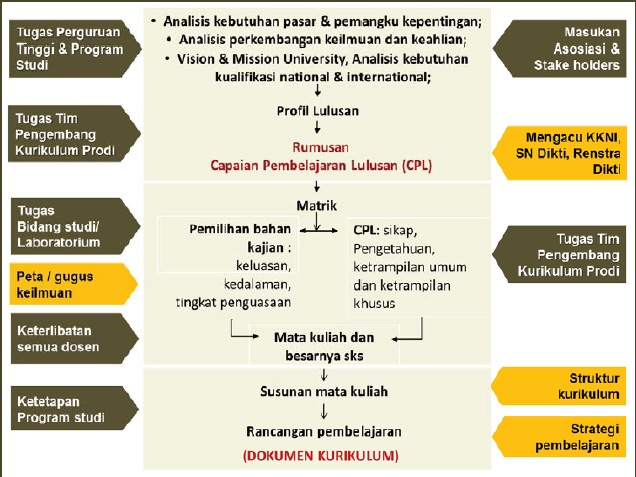
\includegraphics[height=6cm]{Gambar/Penyusunan Kurikulum.jpg}
    \caption{Tahapan penyusunan kurikulum}
    \label{fig:gambar1}
\end{figure}

\subsection{Kodifikasi}
Kodifikasi tiap mata kuliah dibuat berdasarkan Peraturan Rektor UNPAR No. III/PRT/2017-03/46 tentang Standar Penyusunan Kurikulum Program Studi di Lingkungan UNPAR. Kode ini terdiri atas 11 dijit, dengan rincian berikut:

\begin{itemize}
    \item 3 digit - kode khas Program Studi: AIF
    \item 2 digit - tahun diberlakukannya kurikulum (2 digit terakhir): 18
    \item 1 digit - urutan tahun pengajaran
    \item 1 digit - nomor urut KBI pengampu mata kuliah
    \item 2 digit - nomor urut mata kuliah per semester, dengan angka pada dijit terakhir sebagai penentu semester; ganjil atau genap
    \item 2 digit - jumlah sks mata kuliah
\end{itemize}

Informasi lengkap terkait kodifikasi ini diberikan di Gambar \ref{fig:gambar2}.

\begin{figure}[H]
    \centering
    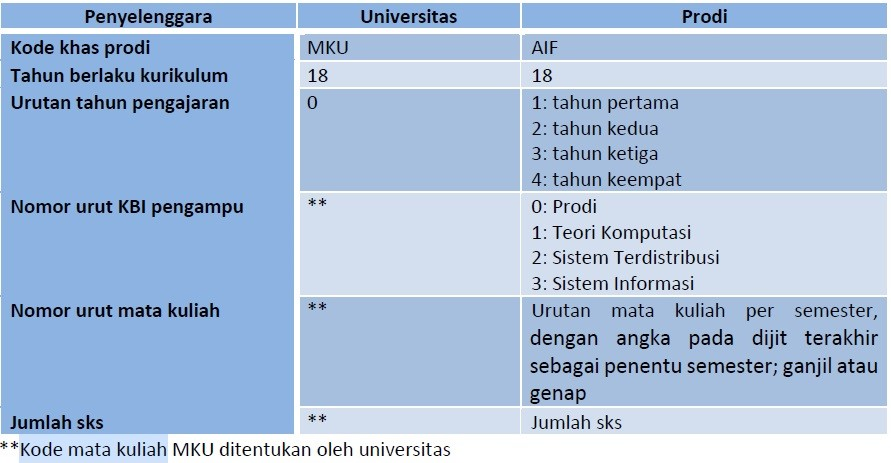
\includegraphics[width=14cm, height=7cm]{Gambar/Kode mata kuliah.jpg}
    \caption{Kodifikasi mata kuliah}
    \label{fig:gambar2}
\end{figure}

\subsection{Bobot Pemrograman}
Berdasarkan hasil evaluasi Kurikulum 2013, salah satu masalah yang ditemukan adalah bahwa mahasiswa masih sulit menguasai materi kuliah di jalur pemrograman, yang merupakan kuliah inti dari Prodi Teknik Informatika UNPAR. Selain karena memang logika pemrograman tidak mudah untuk dipahami, kurangnya pengalaman mahasiswa dalam membangun program komputer juga menjadi penyebab munculnya permasalahan ini. \cite{kurikulum:2018}

Selain memperbaiki struktur kuliah jalur pemrograman, dan perbaikan materi perkuliahan, cara lain yang digunakan untuk mendukung kemampuan pemrograman mahasiswa adalah dengan menempatkan bobot pemrograman di kuliah-kuliah yang cocok. Bobot pemrograman ini menentukan di kuliah mana saja mahasiswa harus membangun program komputer, dan seberapa besar skala program komputer yang
dibuat. Bagian pembangunan program komputer misalnya dapat diletakkan pada saat praktikum, atau dijadikan bagian dari tugas kuliah.
\newpage
Besar bobot pemrograman dalam kurikulum ini adalah 0.25, 0.5, 0.75, dan 1. Penjelasan terkait masing - masing
bobot ini diberikan pada Gambar \ref{fig:gambar3}.

\begin{figure}[H]
    \centering
    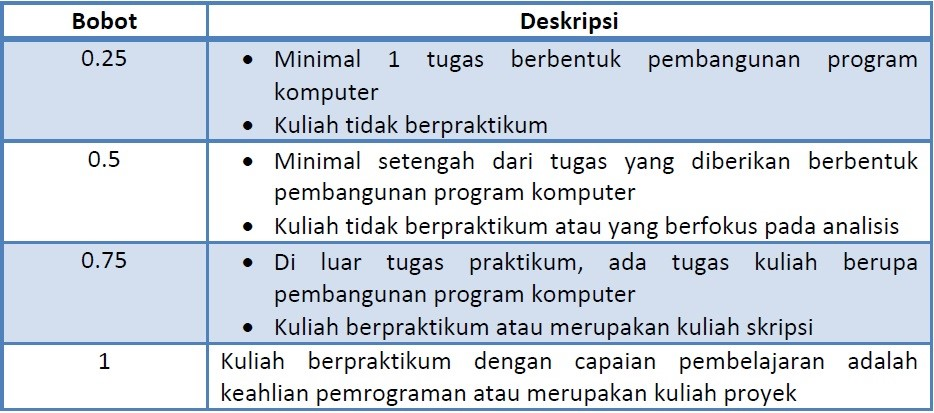
\includegraphics[width=12cm, height=5cm]{Gambar/Bobot Pemorgraman .jpg}
    \caption{Rincian Bobot Pemrograman}
    \label{fig:gambar3}
\end{figure}

\subsection{Prasyarat Mata Kuliah}
Di Prodi Teknik Informatika terdapat 2 jenis prasyarat, yaitu prasyarat lulus dan prasyarat tempuh. Prasyarat lulus artinya seorang mahasiswa harus lulus mata kuliah prasyarat (nilai minimum D), baru dapat mengambil suatu mata kuliah, sedangkan prasyarat tempuh artinya seorang mahasiswa harus pernah menempuh mata kuliah prasyarat, sebelum dapat mengambil suatu mata kuliah. Rincian prasyarat mata kuliah wajib diberikan pada Gambar \ref{fig:gambarSem1}, Gambar \ref{fig:gambarSem2}, Gambar \ref{fig:gambarSem3}, Gambar \ref{fig:gambarSem4}, Gambar \ref{fig:gambarSem5}, Gambar \ref{fig:gambarSem6}, Gambar \ref{fig:gambarSem7}, dan Gambar \ref{fig:gambarSem8}, sedangkan rincian prasayarat mata kuliah pilihan diberikan pada Gambar \ref{fig:gambar11}, Gambar \ref{fig:gambar12}, Gambar \ref{fig:gambar13}, dan Gambar \ref{fig:gambar14}.

\begin{figure}[H]
    \centering
    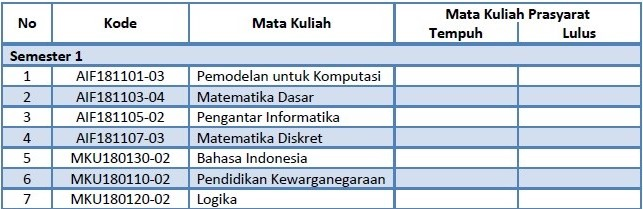
\includegraphics[width=12cm, height=4cm]{Gambar/Prasyarat MK Wajib Sem 1.jpg}
    \caption{Daftar mata kuliah wajib semester satu beserta prasyaratnya}
    \label{fig:gambarSem1}
\end{figure}

\begin{figure}[H]
    \centering
    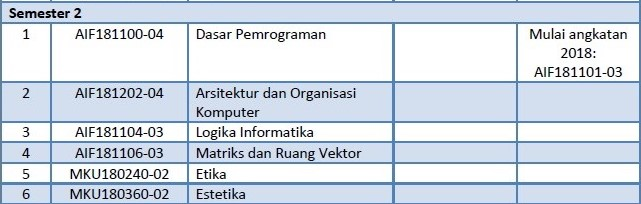
\includegraphics[width=12cm, height=4cm]{Gambar/Prasyarat MK Wajib Sem 2.jpg}
    \caption{Daftar mata kuliah wajib semester dua beserta prasyaratnya}
    \label{fig:gambarSem2}
\end{figure}

\begin{figure}[H]
    \centering
    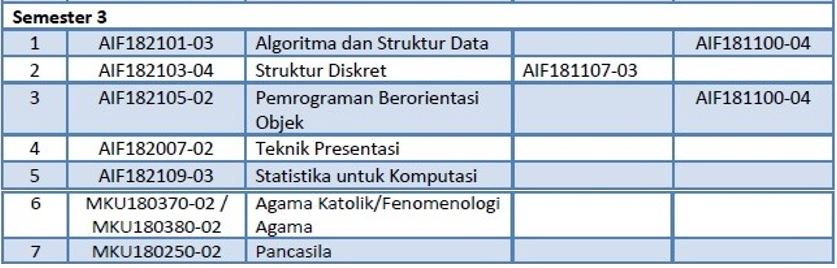
\includegraphics[width=12cm, height=4cm]{Gambar/Prasyarat MK Wajib Sem 3.jpg}
    \caption{Daftar mata kuliah wajib semester tiga beserta prasyaratnya}
    \label{fig:gambarSem3}
\end{figure}

\begin{figure}[H]
    \centering
    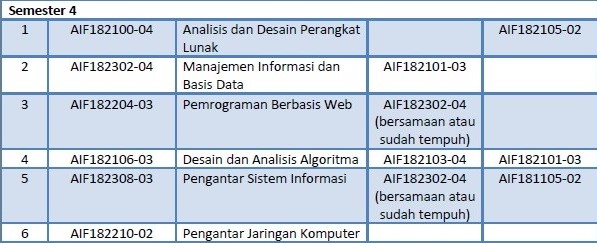
\includegraphics[width=12cm, height=4.5cm]{Gambar/Prasyarat MK Wajib Sem 4.jpg}
    \caption{Daftar mata kuliah wajib semester empat beserta prasyaratnya}
    \label{fig:gambarSem4}
\end{figure}

\begin{figure}[H]
    \centering
    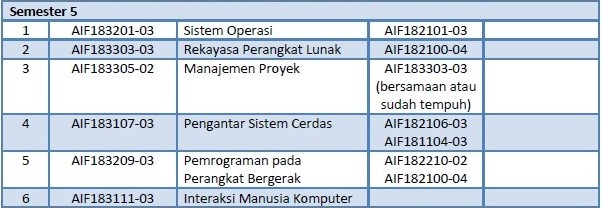
\includegraphics[width=12cm, height=4cm]{Gambar/Prasyarat MK Wajib Sem 5.jpg}
    \caption{Daftar mata kuliah wajib semester lima beserta prasyaratnya}
    \label{fig:gambarSem5}
\end{figure}

\begin{figure}[H]
    \centering
    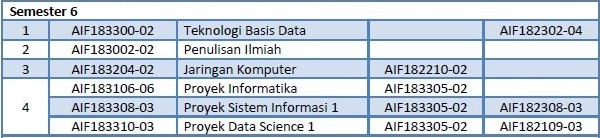
\includegraphics[width=12cm, height=3cm]{Gambar/Prasyarat MK Wajib Sem 6.jpg}
    \caption{Daftar mata kuliah wajib semester enam beserta prasyaratnya}
    \label{fig:gambarSem6}
\end{figure}

\begin{figure}[H]
    \centering
    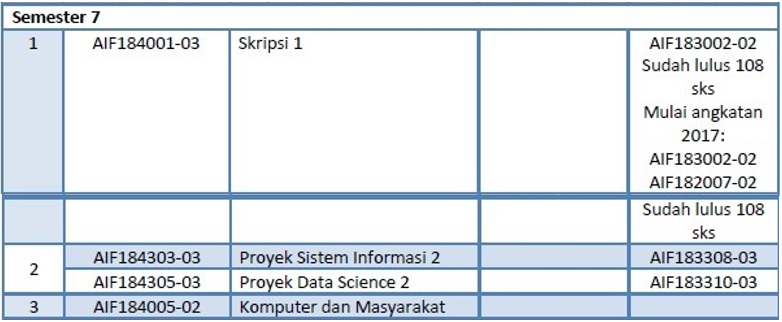
\includegraphics[width=13cm, height=5cm]{Gambar/Prasyarat MK Wajib Sem 7.jpg}
    \caption{Daftar mata kuliah wajib semester tujuh beserta prasyaratnya}
    \label{fig:gambarSem7}
\end{figure}

\begin{figure}[H]
    \centering
    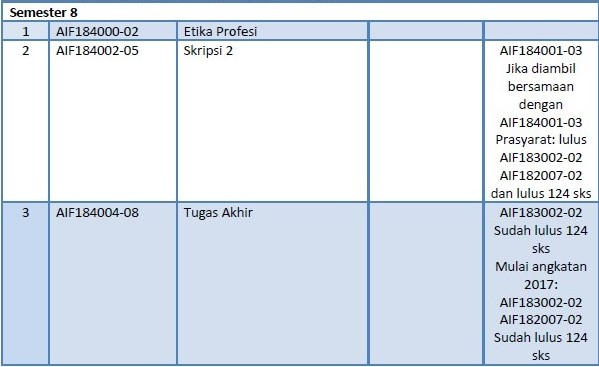
\includegraphics[width=13cm, height=6.5cm]{Gambar/Prasyarat MK Wajib Sem 8.jpg}
    \caption{Daftar mata kuliah wajib semester delapan beserta prasyaratnya}
    \label{fig:gambarSem8}
\end{figure}




\begin{figure}[H]
    \centering
    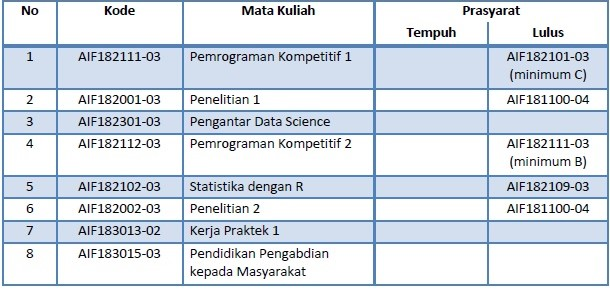
\includegraphics[width=13cm, height=6cm]{Gambar/Prasyarat MK Pilihan 1.jpg}
    \caption{Daftar mata kuliah pilihan beserta prasyaratnya (1)}
    \label{fig:gambar11}
\end{figure}

\begin{figure}[H]
    \centering
    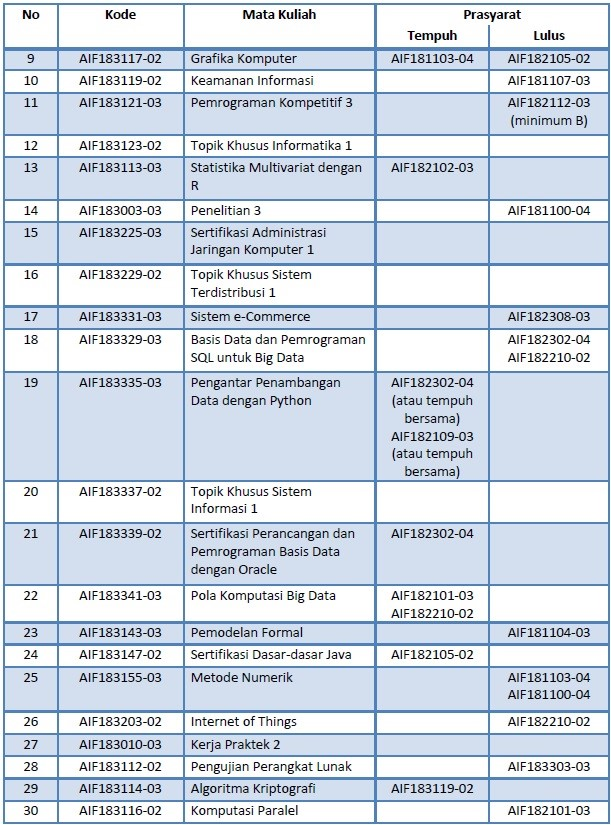
\includegraphics[width=12cm, height=16cm]{Gambar/Prasyarat MK Pilihan 2.jpg}
    \caption{Daftar mata kuliah pilihan beserta prasyaratnya (2)}
    \label{fig:gambar12}
\end{figure}

\begin{figure}[H]
    \centering
    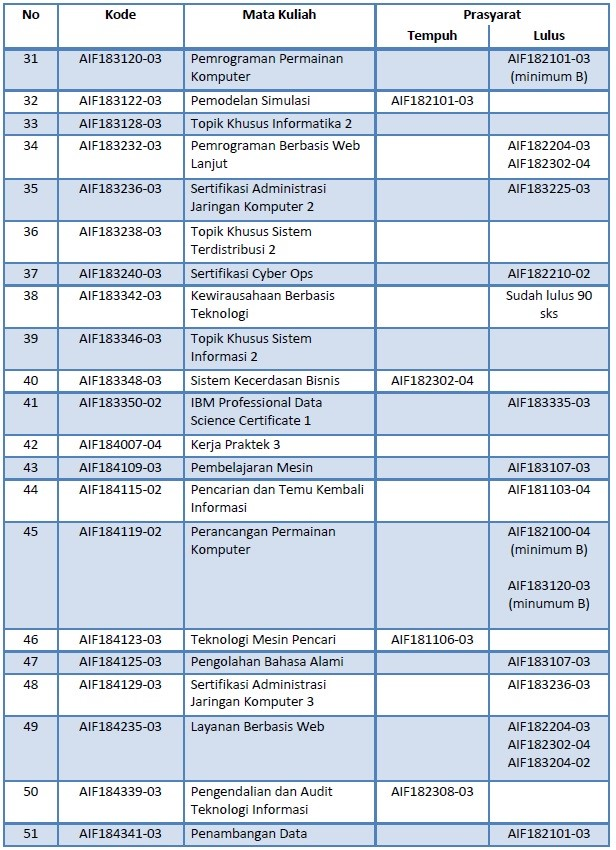
\includegraphics[width=12cm, height=16cm]{Gambar/Prasyarat MK Pilihan 3.jpg}
    \caption{Daftar mata kuliah pilihan beserta prasyaratnya (3)}
    \label{fig:gambar13}
\end{figure}

\begin{figure}[H]
    \centering
    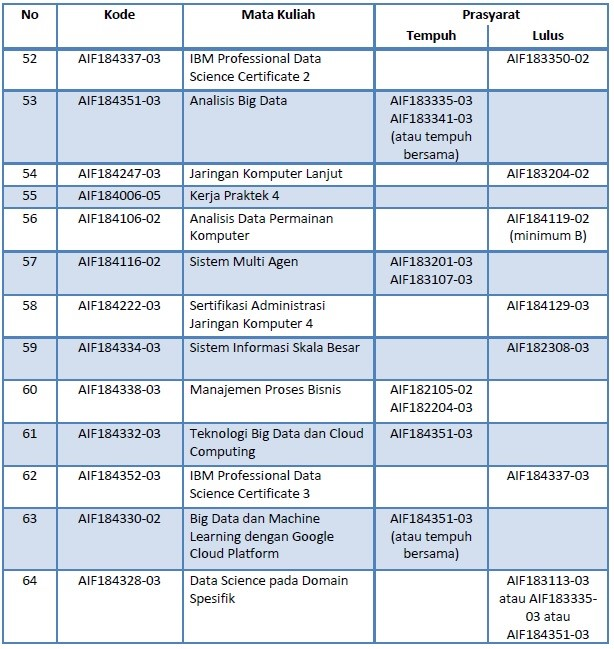
\includegraphics[width=12cm, height=12cm]{Gambar/Prasyarat MK Pilihan 4.jpg}
    \caption{Daftar mata kuliah pilihan beserta prasyaratnya (4)}
    \label{fig:gambar14}
\end{figure}

\newpage
\section{Electron}
\textit{Electron} adalah sebuah \textit{framework} untuk membangun aplikasi \textit{desktop} menggunakan \textit{JavaScript}, \textit{HTML}, dan \textit{CSS}. Dengan menyematkan \textit{Chromium} dan \textit{Node.js} ke dalam binernya, \textit{Electron} memungkinkan kita untuk mempertahankan satu basis kode \textit{JavaScript} dan membuat aplikasi lintas \textit{platform} yang berfungsi di \textit{Windows}, \textit{macOS}, dan \textit{Linux}, dimana tidak diperlukan pengalaman \textit{native} \textit{development}. \cite{electron}

\textit{Electron} mewarisi arsitektur \textit{multi-process} dari \textit{Chromium}, yang membuat kerangka kerja secara arsitektur sangat mirip dengan \textit{browser web} moderen. Selanjutnya, akan dijelaskan konsep pengetahuan tentang \textit{Electron}.

Browser web merupakan sebuah aplikasi yang sangat rumit. Selain kemampuan utama mereka untuk menampilkan konten web, mereka memiliki banyak tanggung jawab sekunder, seperti mengelola beberapa jendela atau tab dan memuat ekstensi pihak ketiga. Pada hari - hari sebelumnya, browser biasanya menggunakan satu proses untuk semua fungsi ini. Meskipun pola ini lebih sedikit \textit{overhead} untuk setiap tab yang dibuka, itu juga berarti bahwa satu situs web yang mogok atau macet akan memengaruhi seluruh browser.

Untuk mengatasi masalah tersebut, tim \textit{Chrome} memutuskan  bahwa setiap tab akan melakukan \textit{render} untuk setiap prosesnya masing - masing, membatasi bahaya yang dapat ditimbulkan oleh kode berbahaya pada halaman web pada aplikasi secara keseluruhan. Satu proses browser kemudian mengontrol proses ini, serta siklus hidup aplikasi secara keseluruhan. Gambar \ref{fig:gambar15} dari \textit{Komik Chrome} memvisualisasikan model ini:

\begin{figure}[H]
    \centering
    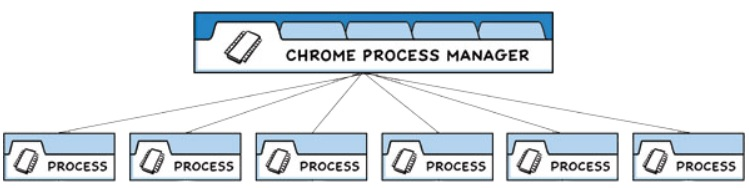
\includegraphics[]{Gambar/Rendered Processes.jpg}
    \caption{Proses \textit{render Chrome}}
    \label{fig:gambar15}
\end{figure}

Aplikasi \textit{Electron} terstruktur sangat mirip. Sebagai pengembang aplikasi, kita mengontrol dua jenis proses : \textit{main} dan \textit{renderer}. Ini adalah analog dengan browser Chrome dan proses \textit{renderer} yang telah diuraikan di atas. Setiap aplikasi \textit{Electron} memiliki satu proses utama, yang bertindak sebagai titik masuk aplikasi. Proses utama berjalan di lingkungan Node.js, artinya ia memiliki kemampuan untuk membutuhkan modul dan menggunakan semua \textit{Node.js APIs}.

Tujuan dari proses utama adalah untuk membuat dan mengelola jendela aplikasi dengan modul \textit{BrowserWindow}. Setiap contoh dari kelas \textit{BrowserWindow} membuat jendela aplikasi yang memuat halaman web dengan proses \textit{renderer} yang terpisah. Kita dapat berinteraksi dengan konten web ini dari proses utama menggunakan  jendela objek webContents. Contohnya dapat dilihat pada Kode \ref{lst:kodeBrowserWindow}.

\begin{lstlisting}[language=JavaScript, caption=Contoh kode penggunaan BrowserWindow\label{lst:kodeBrowserWindow}]
const { BrowserWindow } = require('electron')

const win = new BrowserWindow({ width:800, height: 1500})
win.loadURL('https://github.com')

const contents = win.webContents
console.log(contents)
\end{lstlisting}


Karena modul \textit{BrowserWindow} adalah \textit{EventEmitter}, kita juga dapat menambahkan \textit{handlers} untuk berbagai aktivitas pengguna (misalnya, meminimalkan atau memaksimalkan jendela). Saat instance \textit{BrowserWindow} dimusnahkan, proses \textit{renderer} yang terkait akan dihentikan.

Proses utama juga mengontrol siklus hidup aplikasi melalui modul aplikasi \textit{Electron}. Modul ini menyediakan serangkaian besar kejadian dan metode yang dapat digunakan untuk menambahkan perilaku aplikasi khusus (misalnya, menutup aplikasi secara terprogram, atau memodifikasi dokumentasi aplikasi). Contohnya, pada Kode \ref{lst:kodeKeluarAplikasi} menggunakan API aplikasi untuk membuat pengalaman aplikasi \textit{window} menjadi lebih nyata.

\begin{lstlisting}[language=JavaScript, caption=Contoh kode untuk keluar dari aplikasi\label{lst:kodeKeluarAplikasi}]
app.on('window-all-closed', function(){
    if(process.platform !== 'darwin') app.quit()
})
\end{lstlisting}

Setiap aplikasi \textit{Electron} memunculkan proses penyaji terpisah untuk setiap \textit{BrowserWindow} yang terbuka. Seperti namanya, perender bertanggung jawab untuk merender konten web. Untuk semua maksud dan tujuan, kode yang dijalankan dalam proses perender harus berperilaku sesuai dengan standar web (setidaknya sejauh yang dilakukan Chromium). Oleh karena itu, semua pengguna \textit{interface} dan fungsionalitas aplikasi dalam satu jendela browser harus ditulis dengan alat dan paradigma yang sama dengan yang digunakan di web. Terdapat beberapa spesifikasi web yang harus dipahami, seperti :

\begin{itemize}
    \item File HTML untuk proses rendering.
    \item Menambahkan styling UI melalui Cascading Style Sheets (CSS).
    \item Kode JavaScript yang dapat dieksekusi dengan menambahkannya pada elemen <script>.
\end{itemize}

Maka dari itu, perender tidak memiliki akses langsung ke \textit{require} atau Node.js APIs yang lain. Untuk menyertakan modul NPM secara langsung di perender, kita harus menggunakan \textit{bundler toolchains} yang sama (misalnya, webpack atau parcel) yang digunakan di web.

Untuk cara membuat aplikasi dengan \textit{electron} adalah sebagai berikut :

\begin{enumerate}
    \item Install terlebih dahulu Node.js dan npm (pakai versi terakhir LTS yang tersedia).
    \item Cek versinya dengan mengetik node -v dan npm -v pada command prompt.
    \item Buat folder dan inisialisasi paket npm dengan mengetik mkdir namaFolder lalu ketik cd namaFolder setelah itu ketik npm init pada \textit{command prompt}. Maka isi \textit{package.json} akan seperti pada Kode \ref{lst:kodePackageJson}.
    
    \begin{lstlisting}[language=JavaScript, caption=Package.json\label{lst:kodePackageJson}]
    {
        "name": "my-electron-app",
        "version": "1.0.0",
        "description": "Hello World!",
        "main": "main.js",
        "author": "Jane Doe",
        "license": "MIT",
    }
    \end{lstlisting}
    \item Install aplikasi \textit{electron} ke dalam folder yang telah dibuat dengan cara mengetik npm install --save-dev electron pada command prompt.
    \item Pada \textit{script file} package.json tambahkan \textit{command start} seperti pada Kode \ref{lst:kodeStartCommand}.
    
    \begin{lstlisting}[language=JavaScript, caption=\textit{Start command}\label{lst:kodeStartCommand}]
    {
        "scripts": {
            "start": "electron ."
        }
    }
    \end{lstlisting}
    \item Jalankan aplikasi \textit{electron} dengan mengetik npm start pada command prompt.
\end{enumerate}

\newpage
\section{Vis.js}
\textit{Vis.js} adalah sebuah visualisasi \textit{library} berbasis \textit{browser} yang dinamis. \textit{Library} dirancang agar mudah digunakan, untuk menangani sejumlah besar data dinamis, dan memungkinkan untuk manipulasi dan berinteraksi dengan data. \textit{Library} tersebut terdiri dari komponen \textit{DataSet}, \textit{Timeline}, \textit{Network}, \textit{Graph2d} dan \textit{Graph3d}. \cite{visjs}

\subsection{Timeline}
\textit{Timeline} adalah grafik visualisasi interaktif untuk memvisualisasikan data dalam bentuk waktu. Item data dapat berlangsung pada satu tanggal, atau memiliki tanggal mulai dan berakhir. Kita dapat dengan bebas memindahkan dan memperbesar \textit{timeline} dengan menyeret dan menggulir di \textit{timeline}. Item dapat dibuat, diedit, dan dihapus di \textit{timeline}. Skala waktu pada sumbu disesuaikan secara otomatis, dan mendukung skala mulai dari milidetik hingga tahun. \textit{Timeline} menggunakan HTML DOM biasa untuk merender \textit{timeline} dan item yang diletakkan di \textit{timeline}. Hal ini memungkinkan penyesuaian yang fleksibel menggunakan \textit{css style}. Contoh kode berikut pembuatan \textit{timeline} dapat dilihat pada Kode \ref{lst:kodeTimeline} dan untuk hasilnya dapat dilihat pada gambar \ref{fig:gambarHasilTimeline}.

\begin{lstlisting}[language=HTML, caption=Contoh kode untuk membuat \textit{timeline} menggunakan \textit{vis.js}\label{lst:kodeTimeline}]
<!DOCTYPE HTML>
<html>
<head>
  <title>Timeline | Basic demo</title>

  <style type="text/css">
    body, html {
      font-family: sans-serif;
    }
  </style>

  <script src="../../dist/vis.js"></script>
  <link href="../../dist/vis-timeline-graph2d.min.css" rel="stylesheet" type="text/css" />
</head>
<body>
<div id="visualization"></div>

<script type="text/javascript">
  // DOM element where the Timeline will be attached
  var container = document.getElementById('visualization');

  // Create a DataSet (allows two way data-binding)
  var items = new vis.DataSet([
    {id: 1, content: 'item 1', start: '2013-04-20'},
    {id: 2, content: 'item 2', start: '2013-04-14'},
    {id: 3, content: 'item 3', start: '2013-04-18'},
    {id: 4, content: 'item 4', start: '2013-04-16', end: '2013-04-19'},
    {id: 5, content: 'item 5', start: '2013-04-25'},
    {id: 6, content: 'item 6', start: '2013-04-27'}
  ]);

  // Configuration for the Timeline
  var options = {};

  // Create a Timeline
  var timeline = new vis.Timeline(container, items, options);
</script>
</body>
</html>
\end{lstlisting}

\begin{figure}[H]
    \centering
    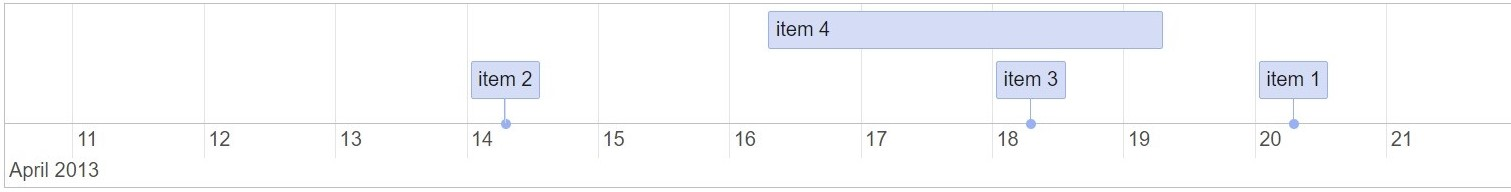
\includegraphics[width=16cm, height=4cm]{Gambar/hasilTimeline.jpg}
    \caption{Hasil contoh untuk membuat \textit{timeline} menggunakan \textit{vis.js}}
    \label{fig:gambarHasilTimeline}
\end{figure}


\subsection{Network}
Jaringan (\textit{Network}) adalah visualisasi untuk menampilkan jaringan - jaringan yang terdiri dari \textit{node} dan \textit{edge}. Visualisasinya mudah digunakan dan mendukung bentuk kustom, gaya, warna, ukuran, gambar, dan lain - lain. Visualisasi jaringan bekerja dengan lancar di \textit{browser} moderen apapun hingga beberapa ribu \textit{node} dan \textit{edge}. Untuk menangani jumlah node yang lebih besar, jaringan memiliki dukungan pengelompokan. Jaringan menggunakan \textit{HTML canvas} untuk \textit{rendering}.

Untuk menggunakan \textit{vis-network}, kita harus menyertakan file \textit{vis-network.js} dan \textit{vis-network.css} yang dapat diunduh dari visjs.org, atau dengan tautkan dari unpkg.com atau bisa juga dengan \textit{import} dari paket npm. Jika kita menambahkan ini ke aplikasi kita, kita perlu menentukan \textit{node} dan \textit{edgenya}. Kita juga dapat menggunakan \textit{vis.DataSets} untuk pengikatan data dinamis, misalnya, mengubah warna, label, atau pilihan apapun setelah kita menginisialisasi jaringan.

Setelah kita memiliki data, yang kita butuhkan hanyalah \textit{container div} untuk memberi tahu \textit{vis} di mana harus meletakkan jaringan kita. Selain itu, kita dapat menggunakan pilihan objek untuk menyesuaikan banyak aspek jaringan. Contoh kode pembuatan \textit{network}  dimana file \textit{vis-network.js} dimasukkan dengan cara menautkan dari unpkg.com dapat dilihat pada Kode \ref{lst:kodeNetwork} dan untuk hasilnya dapat dilihat pada gambar \ref{fig:gambarHasilNetwork}.

\begin{lstlisting}[language=HTML, caption=Contoh kode untuk membuat \textit{network} menggunakan \textit{vis.js}\label{lst:kodeNetwork}]
<html>
<head>
    <script type="text/javascript" src="https://unpkg.com/vis-network/standalone/umd/vis-network.min.js"></script>

    <style type="text/css">
        #mynetwork {
            width: 600px;
            height: 400px;
            border: 1px solid lightgray;
        }
    </style>
</head>
<body>
<div id="mynetwork"></div>

<script type="text/javascript">
    // create an array with nodes
    var nodes = new vis.DataSet([
        {id: 1, label: 'Node 1'},
        {id: 2, label: 'Node 2'},
        {id: 3, label: 'Node 3'},
        {id: 4, label: 'Node 4'},
        {id: 5, label: 'Node 5'}
    ]);

    // create an array with edges
    var edges = new vis.DataSet([
        {from: 1, to: 3},
        {from: 1, to: 2},
        {from: 2, to: 4},
        {from: 2, to: 5}
    ]);

    // create a network
    var container = document.getElementById('mynetwork');

    // provide the data in the vis format
    var data = {
        nodes: nodes,
        edges: edges
    };
    var options = {};

    // initialize your network!
    var network = new vis.Network(container, data, options);
</script>
</body>
</html>
\end{lstlisting}

\begin{figure}[H]
    \centering
    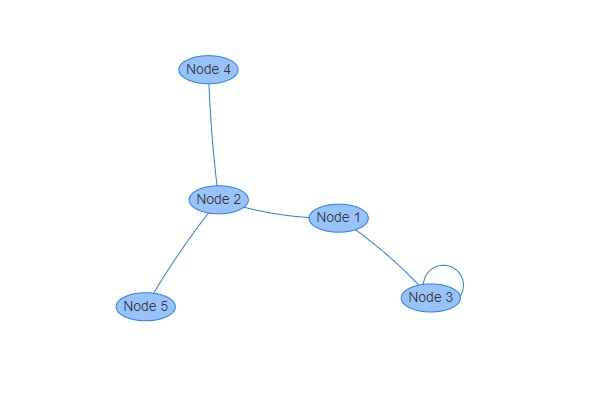
\includegraphics[width=10cm, height=6cm]{Gambar/hasilNetwork.jpg}
    \caption{Hasil contoh untuk membuat \textit{network} menggunakan \textit{vis.js}}
    \label{fig:gambarHasilNetwork}
\end{figure}

\section{FTIS Open Data}
FTIS (Fakultas Teknologi Informasi dan Sains) adalah sebuah fakultas milik UNPAR (Universitas Katolik Parahyangan) yang memiliki tiga program studi, yaitu : Matematika, Fisika, dan Teknik Informatika. \textit{Open data} adalah data yang dapat bebas digunakan oleh semua orang untuk digunakan dan diterbitkan kembali sesuai keinginan, tanpa adanya batasan hak cipta, paten, atau mekanisme kontrol lainnya. Maka dari itu FTIS \textit{Open Data} dapat diartikan sebagai data milik FTIS khususnya program studi teknik informatika yang secara bebas dapat digunakan secara bebas oleh orang lain. FTIS \textit{open data} tersebut dapat diakses pada \url{https://ftisunpar.github.io/data/prasyarat.json}. \cite{ftisOpenData}

\textit{Endpoint} didefinisikan sebagai \textit{url} yang mengikuti setelah basis \textit{url} \url{https://ftisunpar.github.io/data/}. Sebagai contoh \textit{endpoint} prasyarat.json memiliki alamat \textit{url} lengkap \url{https://ftisunpar.github.io/data/prasyarat.json}. Prasyarat.json memiliki informasi tentang seluruh matakuliah, jumlah SKS, posisi semester, serta prasyarat yang ada. Dengan bentuk datanya adalah array dari matakuliah. Setiap struktur matakuliah memiliki properti sebagai berikut : 

\begin{itemize}
    \item kode (String)
    \item nama (String)
    \item prasyarat
    \begin{itemize}
        \item tempuh (String[])
        \item lulus (String[])
        \item bersamaan (String[])
        \item berlakuAngkatan (Number|null)
    \end{itemize}
    \item sks (Number)
    \item wajib (Boolean)
    \item semester (Number)
\end{itemize}

Untuk lebih jelasnya dapat dilihat pada Kode \ref{lst:kodePrasyaratJson}.
\newpage
\begin{lstlisting}[language=JavaScript, caption=prasyarat.json\label{lst:kodePrasyaratJson}]
{
    "kode": "AIF181100",
    "nama": "Dasar Pemrograman",
    "prasyarat": {
      "tempuh": [],
      "lulus": [
        "AIF181101"
      ],
      "bersamaan": [],
      "berlakuAngkatan" : 2018
    },
    "sks": 4,
    "wajib": true,
    "semester": 2
 }
\end{lstlisting}

Pada prasyarat lulus, diberikan sebuah string berupa kode mata kuliah yang menjadi prasyarat lulus untuk mata kuliah tersebut.
Definisi prasyarat berdasarkan macamnya :

\begin{itemize}
    \item Tempuh
    
    Mahasiswa diharuskan sudah pernah menempuh mata kuliah yang disebutkan.
    \item Lulus
    
    Mahasiswa diharuskan untuk lulus mata kuliah yang disebutkan.
    \item Bersamaan
    
    Mata kuliah tersebut harus di ambil secara bersamaan dengan mata kuliah yang disebutkan (butuh informasi lagi).
    \item Berlaku Angkatan
    
    Property ini mulai berlaku karena pergantian kurikulum. Prasyarat ini memiliki maksud bahwa matakuliah ini mulai berlaku semenjak angkatan x.
\end{itemize}




